\chapter{Vehicle Matching Phase}
\section{Methodology for Flight Condition Determination}
\section{Initial MDP Setup}
\subsection{Effect of BLI On MDP Results}
\section{Methodology Implementation on Baseline Vehicle}
\subsection{Baseline Vehicle Requirements}
\subsection{Algorithm Description}
\section{Experiment 5 Results}
\subsection{Baseline Thrust and Stall Margin}
\subsection{Initial BLI Design and Critical Flight Conditions}
\subsection{BLI Re-Design}

	%%
	\begin{figure}[p]
	\centering
	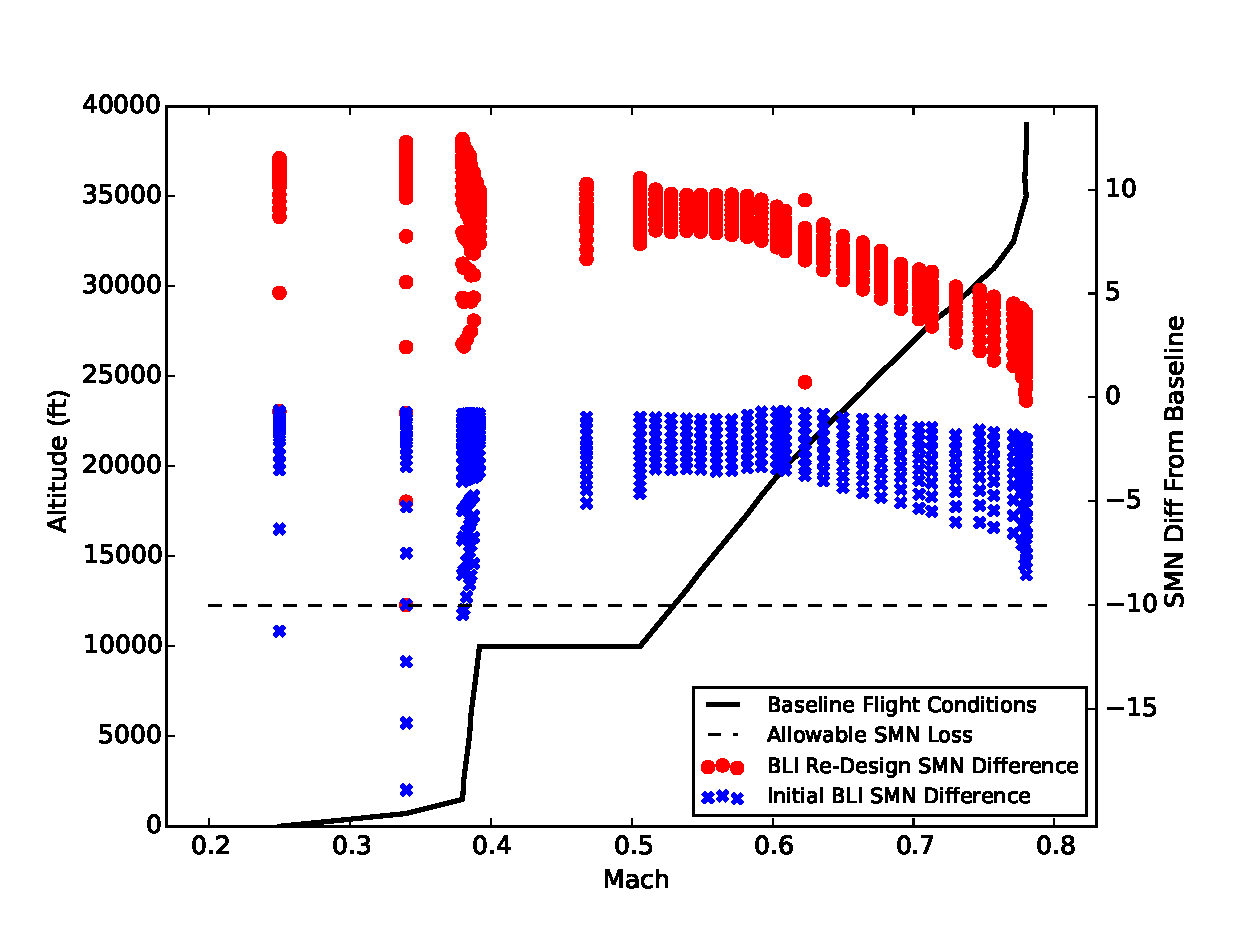
\includegraphics[width=0.8\textwidth]{plot6-5.eps}
	\caption{Angle of attack performance variation for different fidelity models.}
	\label{alpha_sweeps}
	\end{figure}
	%%

\subsection{Impact of BLI Design Variables on Critical Flight Conditions}
\subsection{Impact of Cycle Design Variables on Critical Flight Conditions}
\subsection{Variable Area Nozzle Results}
